\documentclass[conference]{IEEEtran}
\usepackage[utf8]{inputenc}

%\usepackage[portuguese]{babel}
%
%\usepackage{glossaries}  
%\setacronymstyle{short-long}
%
%\newacronym{mpls}{MPLS}{Multiprotocol Label Switching}
%\newacronym{asic}{ASIC}{Application-specific Integrated Circuit}
%
%\makeglossaries

\usepackage{multirow}

\usepackage[pdftex]{graphicx}
\graphicspath{{./Imagens/}}

% correct bad hyphenation here
\hyphenation{op-tical net-works semi-conduc-tor DEFCON}
%

\begin{document}
\title{Wireless Personal Area Networks\\
  \large Redes de Comunicações Móveis\\
  2016/2017
}

\author{\IEEEauthorblockN{Fábio Teixeira}
\IEEEauthorblockA{Faculdade de Ciências da\\Universidade do Porto\\Email: up201305725@fc.up.pt}
\and
\IEEEauthorblockN{Vanessa Silva}
\IEEEauthorblockA{Faculdade de Ciências da\\Universidade do Porto\\Email: up201305731@fc.up.pt}
}

\maketitle

% As a general rule, do not put math, special symbols or citations
% in the abstract
\begin{abstract}

Uma WPAN é uma coleção em rede de dispositivos situados dentro de um curto intervalo (10 metros é muitas vezes um raio de referência). Este tipo de rede serve geralmente para ligar periféricos (impressoras, telemóveis, aparelhos domésticos, etc.) ou permitir a ligação sem fios entre duas máquinas muito pouco distantes. Os baixos custos e consumos de energias e a utilização de pacotes de tamanho reduzido são alguns dos principais objetivos do projeto. Os sistemas WPAN usam links sem fios sem licença, pois esta é a única maneira de conseguir conectividade onipresente sem impacto adverso numa infra-estrutura sem fios.

\end{abstract}


\IEEEpeerreviewmaketitle


\section{Introdução}

O \textit{IEEE 802 Local and Metropolitan Area Network Standards Committee} formou, em março de 1999, um \textit{Working Group} com o intuito de desenvolver padrões de comunicação para redes de área pessoal sem fios. 
O grupo ficou designado por \textit{Project 802.15 Working Group for Wireless Personal Area Networks} (WPANs™) e visava abordar os requisitos que as WPANs necessitavam para possibilitarem comunicação entre dispositivos de computação (especialmente móveis), como PCs, PDAs, telemóveis ou dispositivos eletrónicos (impressoras, por exemplo).

AS WPANs são particularmente aplicáveis em cenários que exigem baixa taxa de transferência de dados, alcance limitado, baixo consumo de energia e que os dispositivos sejam fisicamente pequenos e de baixo custo.

Como as pessoas usam mais dispositivos eletrónicos em casa e no escritório, e com a proliferação de periféricos, cedo se percebeu o sucesso que seria a implementação de conectividade sem fios e que o mercado para estas redes se expandiria rapidamente.

Neste artigo, vamos analisar o estado da arte das WPANs e algumas das tecnologias associadas, nomeadamente, Bluetooth, IrDA e ZigBee.
Este artigo está organizado da seguinte forma.
Primeiramente apresentamos o conceito das WPAN, principais motivações e objetivo, na Secção \ref{conc_mot_obj}.
Na Secção \ref{func_hard} apresentamos o funcionamento destas redes sem fio, assim como uma breve explicação do que são redes \textit{Ad Hoc} e das tecnologias subjacentes que são apresentadas (Bluetooth, IrDA e ZigBee) na Secção seguinte (\ref{arquiteturas}).
Nesta Secção é apresentada, para cada tecnologia, o seu funcionamento e requisitos.
Por último apresentamos algumas conclusões sobre o trabalho de pesquisa realizado (Secção \ref{conclusoes}).


\section{Conceito, Motivação, Objetivos} \label{conc_mot_obj}

\subsection{Conceito}

Uma \textit{Wireless Personal Area Network} (WPAN) é uma rede de área pessoal (\textit{Personal Area Network} (PAN)) que permite conectar dispositivos, (como PCs, PDAs, telemóveis e impressoras), centrados na área (curta) de uma pessoa (ou dispositivo pessoal), com base em conexões sem fio (\textit{Wireless}). 
Deste modo, WPAN forma uma "bolha" wireless em torno de uma "pessoa", conhecida como \textit{Personal Operating Space} (POS) \cite{prasad2004ofdm}, e essa bolha pode, dinamicamente, expandir-se e contrair-se consoante as necessidades.

Além da conexão entre os dispositivos pessoais, que formam a bolha, WPANs devem fornecer ao utilizador uma conexão \textit{ad hoc} (\ref{redes_ad_hoc}) com os recursos e aplicações compatíveis que entram no seu POS \cite{prasad2004ofdm}.
Esta permite que os dispositivos pessoais se comuniquem com outros dispositivos em que a faixa de comunicação interceta o seu POS.

O paradigma das comunicações tradicionais destina-se a estabelecer ligações de comunicação entre dispositivos, enquanto que as WPANs destinam-se a estabelecer comunicações entre pessoas, (dispositivos pessoais habilitados para comunicação), e recursos funcionais/dados através de um meio sem fio (substituindo o tradicional "cabo").

As WPANs são projetadas para operarem na banda mundial ISM (\textit{Industrial}, \textit{Scientific} e \textit{Medical}) de 2,4 GHz. Esta banda proporciona disponibilidade geral em todo o mundo e adequação a soluções de rádio de baixo custo, baixo consumo de energia, curto alcance e não exige a necessidade de uma licença \cite{marsan2002optimizing}, \cite{braley2000wireless}.


\subsection{Motivação}

A motivação para tais redes vem da necessidade da troca de dados não só em grandes distâncias (que é tradicionalmente referida como comunicações), mas também entre pessoas que estão em uma "conversação" em uma curta distância (normalmente até um limite de 10 metros), assim como da necessidade dessa troca de dados ser realizada em um meio sem fio.


\subsection{Objetivos}

Os principais objetivos das WPANs são \cite{prasad2004ofdm}:

\begin{itemize}

 \item Baixo consumo de energia - problema crítico, dado que a velocidade com que o desempenho da bateria melhora é bastante lenta, em comparação com o explosivo crescimento das comunicações sem fio;
 \item Operação no espectro não licenciado - WPANs usam ligações sem fio não licenciadas, uma vez que esta é a única forma de conseguirem conectividade onipresente sem impacto adverso em uma infraestrutura sem fio existente;
 \item Baixo custo;
 \item Pequeno tamanho de pacote.
 
\end{itemize}


\section{Funcionamento, Hardware} \label{func_hard}

\subsection{Funcionamento}

Uma WPAN deve suportar as seguintes operações (inter-relacionadas) \cite{prasad2004ofdm}:

\begin{itemize}

 \item Descoberta de serviço - os dispositivos devem ter a capacidade de descobrirem o recurso de serviço ou informação necessária;
 \item Estabelecimento de conexão \textit{ad hoc} - os dispositivos devem ter a capacidade de estabelecerem uma conexão \textit{ad hoc} com o dispositivo que oferece esse serviço ou contém esse recurso.
 
\end{itemize}

A descoberta de serviço permite que um dado dispositivo tenha acesso ao serviço que está disponível dentro do seu intervalo de comunicação (POS).
Por exemplo, um dado PDA, encontra uma impressora dentro do seu intervalo de comunicação, reconhece-o, (descoberta de serviço), como um recurso disponível (desde que certas condições de segurança sejam satisfeitas) e usa-o, (estabelecimento de conexão), como se a impressora fosse instalada no seu \textit{software} \cite{prasad2004ofdm}.

\subsection{Redes \textit{Ad Hoc}} \label{redes_ad_hoc}

Uma rede \textit{ad hoc} é um tipo de rede sem fio constituída por nós que cooperam entre si de forma a encaminharem pacotes na rede (determinam quando um nó pode transmitir e receber dados), sem a necessidade de uma infraestrutura de forma a que cada nó possa comunicar diretamente com outro nó \cite{salonidis2005distributed}, \cite{rubinstein2002qualidade}. 
Esta comunicação (de um nó A para um nó B) só pode ser estabelecida se o nó B estiver dentro do raio de ação (locais onde o sinal chega com clareza) de A ou então, se existir um ou mais nós entre A e B que possam encaminhar os dados.

Em termos de roteamento, toda a rede é baseada na ideia de que os dispositivos funcionarem tanto como \textit{routes} e como \textit{hosts} \cite{prasad2004ofdm}.


\subsection{Tecnologias Associadas}

Existem várias tecnologias \textit{standard} que fornecem conectividade sem fio em curtas distâncias. 
Destacamos as seguente, \textbf{Bluetooth}, \textbf{IrDA}, \textbf{Zigbee}, \textbf{HomeRF} e \textbf{UWB}, onde analisamos apenas algumas destas, na secção (\ref{arquiteturas}).
Embora cada uma destas tecnologias tenha atingido aplicações e modelos de uso diferentes, o princípio por detrás de todas é a utilização de algum tipo de tecnologia de rádio subjacente, de forma a permitir a transmissão sem fio de dados, fornecer suporte para a formação de redes e gerenciar vários dispositivos através de \textit{software} de alto nível \cite{prasad2004ofdm}.


\section{Modelos de Arquitetura/\textit{standard}} \label{arquiteturas}

\subsection{Bluetooth} \label{bluetooth}

O Bluetooth, também conhecido por IEEE 802.15.1, é um tipo de tecnologia WPAN sem fio, que estabelece uma comunicação de curta distância e baixo custo. 
Tem como objetivo o estabelecimento de conexões e troca de informação entre dispositivos, como telemóveis, computadores, impressoras, câmaras e até consolas de jogos, utilizando para isso uma frequência de rádio de curto alcance. 
Foi lançado em 1994 pela Ericsson, embora outras companhias como a Nokia, a IBM, a Intel e a Toshiba também se tenham juntado à empresa sueca em 1998, formando um grupo chamado Bluetooth SIG (\textit{Special Interest Group}), com o intuito de desenvolver, promover e expandir esta tecnologia. 
Nos dias de hoje, milhares de empresas já se juntaram ao grupo, entre elas estão nomes fortes como a Samsung, a Microsoft, a Motorola, a Dell, a HP, a Phillips, a Siemens e a Texas \cite{bluetoothwiki}.

Algumas das especificações desta importante tecnologia são \cite{kobayashi2004tecnologia}:

\begin{itemize}

 \item Não requer obrigatoriamente linha de vista para funcionar, sendo capaz de comunicar através de barreiras físicas, como é o caso da tecnologia de infravermelhos.
 \item Conta tipicamente com um alcance de 10 metros, embora este valor possa ser amplificado. 
 \item Opera na faixa de licença-livre ISM a aproximadamente 2,45 GHz, com um débito máximo típico de 1 Mbps, que se estima que possa ser aumentado, com futuras especificações.
 \item Divide ainda a faixa de 2,45 GHz em 79 canais e muda de canal, (\textit{Frequency-hopping spread spectrum} (FHSS)), cerca de 1600 vezes por segundo, de forma a evitar possíveis interferências com outros protocolos que usam a mesma faixa.

\end{itemize}

\subsubsection{Funcionamento}

\begin{figure}[!t]
  \centering
  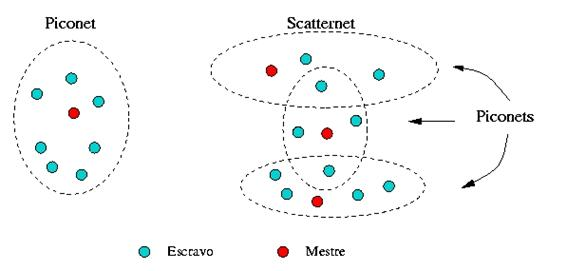
\includegraphics[width=0.45\textwidth]{Esquema_Bluetooth.png}
  \caption{Topologia da tecnologia Bluetooth \cite{blueesptec}.}
  \label{fig:topBluet}
\end{figure}

\begin{figure}[!t]
  \centering
  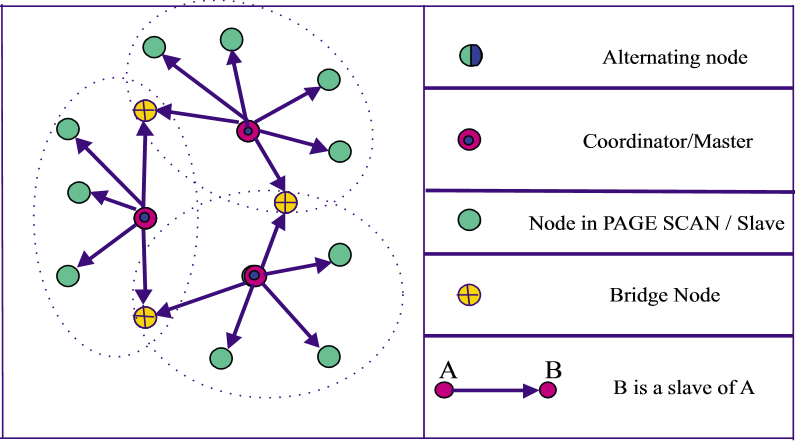
\includegraphics[width=0.45\textwidth]{no_ponte.png}
  \caption{Representação da conexão de três \textit{piconets} atavés de um nó ponte \cite{salonidis2005distributed}.}
  \label{fig:noPonte}
\end{figure}

O Bluetooth baseia-se numa camada física de saltos de frequência (FHSS), que permite que dispositivos portáteis formem redes \textit{ad hoc} sem fio de curto alcance \cite{salonidis2005distributed}. 
Os \textit{hosts} Bluetooth não são capazes de comunicar a menos que se tenham previamente descoberto uns aos outros, através da sincronização dos seus padrões de tempo e frequência. 
Assim, mesmo que todos os nós estejam próximos uns dos outros, apenas os nós que estão sincronizados com o transmissor podem ouvir a transmissão.
Para suportar comunicação \textit{any-to-any}, os nós devem ser sincronizados de modo a que os pares de nós, que se podem comunicar, formem um gráfico conectado.

O sistema de saltos de frequência, define vários canais para comunicação, sendo que cada canal é baseado numa sequência de salto de frequência diferente \cite{salonidis2005distributed}. 
Assim, um grupo de dispositivos que compartilham um mesmo canal, (que se conectam de forma \textit{ad hoc}), é chamado de \textit{piconet}. 

Cada \textit{piconet} tem uma unidade \textbf{mestre} (\textit{master}) que seleciona uma sequência de salto de frequência para o \textit{piconet} e controla o acesso ao canal. 
Os outros participantes do grupo, conhecidos como unidades \textbf{escravas} (\textit{slaves}), são sincronizados com a sequência de salto do \textit{piconet master} \cite{salonidis2005distributed}. 

Dentro de um \textit{piconet}, o canal é compartilhado usando um \textit{slotted Time Division Duplex} (TDD), em que um \textit{master} usa um protocolo de pesquisa para alocar faixas horárias para os \textit{slaves}. O número máximo de \textit{slaves} que podem ser simultaneamente ativos num \textit{piconet} é sete.

Quando os vários \textit{piconets} (lado esquerdo da figura (\ref{fig:topBluet})) são conectados, forma-se uma rede wireless chamada \textit{scatternet}, como ilustrado à direita da figura (\ref{fig:topBluet}).
Isto é possível, pois cada \textit{piconet} utiliza uma sequência de salto diferente, o que faz com que múltiplos \textit{piconets} possam coexistir numa área comum \cite{salonidis2005distributed}, uma vez que esta diferença reduz a interferência mútua a um nível aceitável \cite{prasad2004ofdm}. 
Estes são então conectados através de uns nós especiais, chamados de nós ponte, que podem ser construídos entre dois \textit{masters}, como podemos ver na figura (\ref{fig:noPonte}), entre um \textit{master} e um \textit{slave} ou entre dois \textit{slaves} \cite{salonidis2005distributed}.

Cenário real deste funcionamento seria uma impressora e um PC equipados com Bluetooth. Quando o PC chega ao alcance da impressora, esta dá-se a conhecer para que, quando o usuário desejar imprimir um documento, os dois dispositivos possam iniciar imediatamente a transferência de dados. Enquanto isso, possivelmente, outros PCs, que terão chegado ao alcance destes dispositivos, se unirão à \textit{piconet} estabelecida para que também possam usar a impressora quando necessário.

Dada uma coleção de dispositivos Bluetooth, é necessário um protocolo explícito de construção de topologia para formar \textit{piconets}, atribuir \textit{slaves} a \textit{piconets} e conectar \textit{piconets} através de nós ponte, de modo que o \textit{scatternet} resultante fique conectado. Tal protocolo deve ser assíncrono, distribuído e pode começar com nós que não têm qualquer informação sobre o seu ambiente \cite{salonidis2005distributed}.

\subsubsection{Benefícios}

O consumo de cada transmissor Bluetooth é de aproximadamente 50 mA, dentro do limite de 10 metros, o que representa cerca de 3\% do consumo total de um telemóvel, valor que é quase irrisório comparado com outras tecnologias sem fio. 
Este baixo consumo permite que os dispositivos venham já com a tecnologia de fábrica, sem comprometer a autonomia das baterias. 
Os \textit{developers} do projeto depressa perceberam que muito mais seria possível fazer aproveitando a tecnologia do Bluetooth. 
Se transmitir informação entre um computador e uma impressora era uma realidade, também o poderia ser transmitir dados de um telemóvel para uma impressora, ou mesmo entre impressoras. 
E com o baixo custo de um chip Bluetooth (cerca de 5 euros) e o baixo consumo de energia da tecnologia. 
O número de aplicações e benefícios da tecnologia rapidamente se tornaram inimagináveis \cite{kobayashi2004tecnologia}.

\subsubsection{Classes e Versões}

Existem atualmente 3 classes da tecnologia, numeradas de 1 a 3. 
A classe 1 é a mais potente, permitindo consumos até 100 mW com um alcance de 100 metros. 
A classe 2, por seu lado, possibilita cerca de 2.5 mW de potência máxima, com um alcance de 10 metros. 
Já a classe 3 permite 1 mW de potência, transmitindo numa distância de cerca de 1 metro \cite{bluetoothwiki}.

%o que queres dizer aqui? exisitam???? 
Versões também exisitam 3 até há pouco tempo, mas recentemente foi lançado o Bluetooth 4, que traz vantagens no consumo de energia, velocidade e segurança, entre outros. 
A versão 3 era até então a versão com maior taxa de transmissão, cerca de 24 Mbps, enquanto que as versões 2 e 1.2 se ficavam pelos 3 e 1 Mbps, respetivamente \cite{bluetoothwiki}.

%\subsubsection{Bluetooth vs. Wi-Fi} talves devessemos retirar esta secção já que nao falamos em mais lado nenhum do wifi e assim...

%Resumidamente, embora o Bluetooth utilize a mesma de 2,45 GHz do 802.11b e do 802.11g, o Wi-Fi continua a ser uma melhor opção, já que uma rede Bluetooth é muito mais lenta e, para além de suportar poucos dispositivos, é ainda menos segura. O Wi-Fi, por sua vez, apesar de requerer mais configurações, é melhor para operar redes de alta-escala pelo simples facto de suportar conexões rápidas e seguras com melhor potência de transmissão e receção. %cite{http://www.diffen.com/difference/Bluetooth_vs_Wifi}


\subsection{Infravermelhos - IrDA}

\textit{Infrared Data Association}, também conhecido por IrDA, é uma organização internacional que cria e promove padrões de conexão de dados de infravermelho (IR) de baixo custo e interoperáveis.
Foi criada em 1993 por cerca de 50 empresas e possui um conjunto de protocolos de suporte a uma ampla gama de aparelhos de computação e dispositivos de comunicação. 
Estes protocolos são tipicamente destinados a fornecer altas velocidades, comunicação de curto alcance em linha de vista e transferência ponto-a-ponto de dados sem fios. 
Os protocolos IrDA utilizam o IrDA DATA como mecanismo de entrega de dados e o IrDA CONTROL como mecanismo de controlo \cite{infareddd}.

A motivação original da IrDA visa essencialmente fornecer uma tecnologia que possa substituir a utilização de cabos, bem como de outros padrões PAN. 
A ideia é que dois dispositivos possam comunicar simplesmente apontando-os um para o outro, o que tornaria a utilização de cabos completamente desnecessária. 
A IrDA estima que existam mais de 300 milhões de dispositivos, tornando a comunicação por IR uma das tecnologias sem fios mais difundidas pelo globo terrestre \cite{wpanonline}.

Alguma especificações desta tecnologia são:

\begin{itemize}

 \item Alcance de comunicação de até 1 metro, embora uma distância de 2 metros muitas vezes pode ser alcançada.
 \item Baixa potência para comunicação de até 20 centímetros. Isso requer 10 vezes menos energia do que a implementação completa.
 \item Comunicação bidirecional.
 \item Transmissão de dados de 9600 bps para uma velocidade máxima de 4 Mbps.

\end{itemize}

\subsubsection{Protocolos requeridos}

Uma pilha de protocolos IrDA é o conjunto de camadas de protocolos das comunicações IR ponto-a-ponto. 
Os protocolos de comunicação tratam de várias funcionalidades, e por isso são geralmente partidos em camadas. 
Cada uma destas camadas lida com um conjunto de responsabilidades e fornece recursos necessários para as camadas acima e abaixo \cite{megowan1996irda}.

As camadas necessárias para a pilha de protocolos IrDA são as seguintes:

\begin{itemize}

 \item \textit{Physical Layer}: especifica características óticas, codificação de dados e enquadramento para várias velocidades;
 \item IrLAP (\textit{Link Access Protocol}): estabelece a conexão confiável básica;
 \item IrLMP (\textit{Link Management Protocol}): multiplexa serviços e aplicativos na conexão LAP;
 \item IAS (\textit{Information Access Service}): fornece "páginas amarelas" de serviços num dispositivo.

\end{itemize}

A utilização das camadas opcionais depende da aplicação em particular. Os protocolos opcionais são:

\begin{itemize}

 \item TinyTP (\textit{Tiny Transport Protocol}): adiciona controlo de fluxo por canal para manter as coisas em movimento sem problemas. Esta é uma função muito importante e é necessária em muitos casos;
 \item IrOBEX (\textit{The Object Exchange Protocol}): fácil transferência de arquivos e outros objetos de dados;
 \item IrCOMM: emulação de porta serial e paralela, permitindo que os aplicativos existentes que usam comunicações seriais e paralelas usem o IR sem alterações;
 \item IrLAN (\textit{Local Area Network access}): permite o acesso IR LAN sem fios para \textit{laptops} e outros dispositivos.

\end{itemize}

% Imagem: http://i.imgur.com/c9Kotc3.png (acho que não vou colocar a imagem por questoes de espaço e não ser muito necessária)


\subsubsection{Benefícios}

Uma das principais vantagens da IrDA a partir da perspetiva de um fabricante de dispositivos é o seu baixo custo. 
As portas de infravermelhos podem ser incorporadas num dispositivo por valores inferiores a 1 euro, o que representa um custo muito baixo para a implementação de comunicação sem fios num dispositivo, em comparação com outros padrões WPAN. 
Para além disto, proporcionam maior segurança e independência face às ondas de rádio e o facto de os dispositivos serem leves, consumirem pouco e serem fáceis de usar \cite{infaredadvdis}.


\subsubsection{Limitações}

O uso de IR para transferência de dados é uma excelente ideia, em teoria. 
No entanto, mesmo com esta ubiquidade, a tecnologia raramente é utilizada para satisfazer a sua intenção original, ou seja, a transferência de dados. 
Isto porque, para que o IR funcione, os dispositivos de comunicação têm de estar em linha de vista, o que pode ser um problema em vários cenários. 
Num ambiente de escritório, esta limitação não é prática para muitos periféricos, como impressoras ou \textit{scanners}, que não mantêm a obrigatoriedade de estarem em linha de vista. 
Para além deste problema, o IR também peca pelo facto de os dispositivos não se poderem mover enquanto a transmissão está em progresso e pela ideia de que a maioria dos utilizadores não tem dois dispositivos com portas IR. 
Enquanto quase todos os dispositivos portáteis tem suporte para IrDA, a maioria dos \textit{desktops} não possui esse mesmo suporte, o que limita a eficácia da tecnologia como protocolo de transferência de dados \cite{wpanonline}.


\subsection{IEEE 802.15.4 - ZigBee}

O padrão de comunicação sem fio ZigBee baseia-se no padrão IEEE 802.15.4 LR-WPAN, e foi concebido de forma a possibilitar a interconexão de dispositivos sem fio simples (de frequência de rádio), que requerem baixa taxa de dados, baixa bateria e baixo custo \cite{kennedy2008review}, assim como, redes de eletrodomésticos, monitorização médica, controlo industrial e sensores ambientais.

Este padrão resulta da aliança entre o IEEE e a ZigBee Alliance , em que o primeiro ficou responsável pela criação das duas camada mais baixas da pilha do protocolo ZigBee (camada \textbf{PHY} e \textbf{MAC}), e a segunda pelas camadas superiores (camada \textbf{Network} e \textbf{Application}) \cite{liang2006impact}.

Numa rede ZigBee, cada nó pode ser de dois tipos, segundo o IEEE, dispositivo de função completa (\textit{Full Function Device} (FFD)) ou dispositivo de função reduzida (\textit{Reduced Function Device} (RFD)), dependendo de suas capacidades.
O primeiro pode desempenhar três papeis específicos na rede, o papel de \textit{router} (ou coordenador PAN), (e consequentemente ter acesso a todos os outros dispositivos), o papel de coordenador ou de dispositivo final.
E os segundos, os RFDs, apenas podem desempenhar o papel de dispositivo final, podendo comunicar apenas com os FFDs, (ao contrário dos FFDs que podem comunicar com RFDs ou FFDs) \cite{liang2006impact},\cite{sinem2004zigbee}.
O coordenador é responsável por iniciar uma nova rede e, assim como os \textit{routers}, podem realizar o encaminhamento de dados, ao contrário dos dispositivos finais que não podem participar no encaminamento e têm de "confiar" nos seus \textit{routers} pai \cite{liang2006impact}.


\subsubsection{Funcionamento}

\begin{figure}[!t]
  \centering
  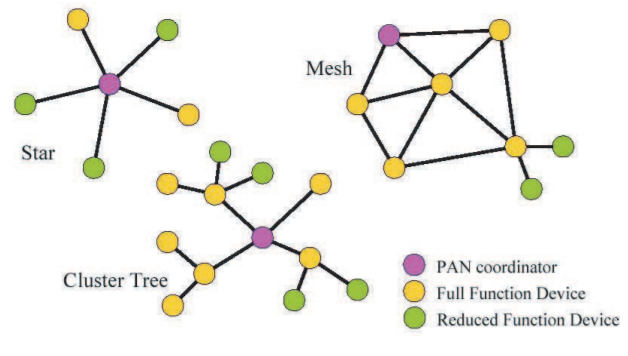
\includegraphics[width=0.45\textwidth]{Modelos_Topologias_ZigBee.png}
  \caption{Modelos de topologias da tecnologia ZigBee \cite{sinem2004zigbee}.}
  \label{fig:topZigBee}
\end{figure}

O esquema de funcionamento de uma rede ZigBee é a chave para se obter a eficiência de recursos pretendida (por exemplo, largura de banda e energia).

Com base nas camadas PHY e MAC, ZigBee estabelece o \textit{framework} para as camadas \textit{Network} e \textit{Application} \cite{liang2006impact}.

Na camada PHY, o IEEE 802.15.4 define um total de 27 canais, dos quais 16 apresentam uma taxa máxima de 250 kbps na banda ISM 2,4-2,4835 GHz (global), que utiliza modulação O-QPSK, 10 apresentam uma taxa máxima de 40 kbps na banda ISM 902-928 MHz (América), e 1 apresenta uma taxa máxima de 20 kbps na banda 868,0-868,6 MHz (Europa), em que estas últimas utilizam modulação BPSK.
Esta camada é responsável por permitir a transmissão de unidades de dados, através de ondas de rádio.
Utiliza a modulação \textit{Direct Sequence Spread Spectrum} (DSSS) que inclui em cada bit de dados um padrão de redundância, (permitindo, não só, que os dados sejam identificados como pertencentes a um determinado nó, como também facilita a deteção de erros), e os espalha pela largura de banda utilizada.
Ao espalhar os dados em todas as frequências da banda, o sinal resultante assemelha-se a um ruído, tornando-se mais robusto a interferências. 
Após ser feita a DSSS, o sinal é modulado em uma portadora e transmitido \cite{liang2006impact}.
%Esta camada é também responsável por indicar a qualidade da conexão (através do valor do pacote \textit{Link Quality} que é calculado pelas camadas superiores de acordo com a relação sinal-ruído (SNR) e o valor do pacote \textit{Energy Detection} (ED)), detetar a potência dos canais (o ED representa em 8 bits a relação em dB da potência recebida nos canais) e indicar canais livres (determina se os canais estão ocupados através do \textit{Carrier Sense} do sinais em DSSS e/ou caso o valor de ED esteja acima do limite do canal). 

Na camada MAC, utiliza-se o \textit{Carrier Sense Multiple Access with Collision Avoidance} (CSMA/CA) e suporte para o modo \textit{beacon} e \textit{non-beacon} \cite{liang2006impact}.
Esta camada é responsável pelo encapsulamento dos dados vindos das camadas superiores preparando-os para serem transmitidos.

Em modo \textit{beacon} os \textit{routers} (FFD) transmitem periodicamente \textit{beacon frames}, (pequenos pacotes que confirmam a sua presença na rede), a outros dispositivos \cite{cirilo2014computaccao}, \cite{liang2006impact}, e todos o nós, à exceção do coordenador, podem permanecer inativos (\textit{sleep}) entre \textit{beacons} economizando energia.
É utilizada a estrutura de \textit{superframe} que promove banda livre em algumas situações e proporciona baixa latência nas transmissões.
Esta é limitada por \textit{beacon frames} a cada período de tempo pré-determinado e o tempo total será igualmente dividido em 16 \textit{slots} de tempo.
Após o \textit{beacon}, é apresentado os tempos de acesso CAP (Contension Access Period), onde todos os dispositivos competem entre si utilizando CSMA-CA, e o tempo livre, CFP (Contension Free Period), que garante \textit{slots} de tempo para cada dispositivo. 
Após isto, o dispositivo entra em modo inativo, economizando energia.

O CSMA-CA consiste em, quando um dispositivo pretende transmitir, primeiro ele "ouve" o canal durante um período de tempo pré-determinado, se o canal estiver livre o dispositivo pode transmitir, caso contrário o dispositivo faz um \textit{backoff} de um período de tempo, reiniciando o processo após esse tempo.

Em modo \textit{non-beacon} é utilizado o \textit{unslotted} CSMA/CA que tem um tempo de espera aleatório, não dependente de \textit{slots}, aqui os \textit{routers} ZigBee normalmente têm seus recetores continuamente ativos, não permitindo economizar energia.
Isto permite redes heterogéneas, nas quais alguns dispositivos recebem continuamente, enquanto outros transmitem apenas quando algum estímulo externo é detetado. 
Um exemplo de uma rede heterogénea é um interruptor de luz sem fio, em que o nó ZigBee na lâmpada recebe constantemente, uma vez que é conectado à rede elétrica, enquanto que um interruptor de luz alimentado por bateria permaneceria inativo (\textit{sleep}) até que o interruptor é acionado, aqui acorda, emite um comando à lâmpada, recebe uma confirmação, e retorna ao estado inativo \cite{zigbee_online}.

Esta rede ZigBee pode ter uma das três topologias seguintes (como pode ser observado na figura \ref{topZigBee}) \cite{sinem2004zigbee}:

\begin{itemize}

 \item \textit{Star} - a comunicação é estabelecida entre os dispositivos (FFDs e/ou RFDs) e um único controlador central (coordenador PAN). Depois que um FFD seja ativado pela primeira vez, ele pode estabelecer a sua própria rede tornando-se o coordenador PAN dela. Cada rede inicial escolhe um identificador PAN, que não é usado por nenhuma rede dentro da suas esfera de rádio. Isso permite que cada rede \textit{star} opere de forma independente. Esta topologia é ideal para automação residencial, computadores pessoais (PC), brinquedos e jogos.
 
 \item \textit{Peer-to-peer} ou \textit{Mesh} - também existe um coordenador PAN, mas aqui qualquer dispositivo pode-se comunicar com qualquer outro, desde que estejam no alcance rádio um do outro. Esta topologia é ideal para aplicações como controle e monitorização industrial e redes de sensores sem fio. 
 
 \item \textit{Cluster-tree} - é um caso especial de uma rede \textit{peer-to-peer}, aqui a maioria dos dispositivos são FFDs. Um RFD pode-se conectar a uma rede \textit{cluster-tree} como um nó de saída no fim de uma ramificação e qualquer um dos FFDs pode atuar como coordenador e fornecer serviços de sincronização para outros dispositivos e coordenadores, mas apenas um desses coordenadores é o coordenador PAN. Este forma o primeiro \textit{cluster} (sendo a cabeça de \textit{cluster} (CLH)) e escolhe um identificador PAN não utilizado. Um dispositivo pode solicitar a adesão à rede ao CLH e se este permitir que o dispositivo se junte, ele irá adiciona-lo como um dispositivo filho na sua lista de vizinho e este adicionará o CLH como seu pai na sua lista de vizinhos e começará a transmitir \textit{beacons} periódicos de modo que outros dispositivos possam aderir à rede nesse novo dispositivo. Uma vez satisfeitos os requisitos da rede, o coordenador PAN pode instruir um dispositivo a se tornar o CLH de um novo \textit{cluster} adjacente ao primeiro. 

\end{itemize}


%tabela de comparações entre tecnologias (possivelmente servirá para reduzirmos texto)
%\begin{table}[h]	%[h]-faz com que a tabela fique neste mesmo sitio
%\centering
%\caption{Tabela de comparação entre as diferentes tecnologias apresentadas.}	%legenda
%\begin{tabular}{l|ccc}

%& \textbf{Bluetooth} & \textbf{IrDA} & \textbf{ZigBee} \\
%\hline

%\textbf{Alcance} & 1-100 m & [1-2 m] & 10-100 m \\
%\hline
%\textbf{Canais} & 79 & [irda] & 27 \\
%\hline
%\multirow{3}{*}{\textbf{Frequência}} & \multirow{3}{*}{2,45 GHz} & [irda] & 2,4-2,4835 GHz \\
%									 &	 						 & [irda] & 868,0-868,6 MHz \\
%									 &	  						 & [irda] & 902-928 MHz \\
%\hline
%\multirow{3}{*}{\textbf{Modulação}} & \multirow{3}{*}{FHSS} & [irda] & O-QPSK \\
%									&		 				& [irda] & BPSK \\
%									&		 				& [irda] & BPSK \\
%\hline
%\textbf{Taxa de Dados (min-max)} & 1 Mbps–24 Mbps & 9.6 kbps-1 Gbps & 20 kpbs–250 kbps \\
%\hline
%\textbf{Canal de Acesso} & FH-CDMA & [irda] & \textit{Slotted}/\textit{Unslotted} CSMA/CA \\
%\hline
%\textbf{Topologia de Rede} & \textit{Piconets}, \textit{Scatternets} & [irda] & \textit{Star}, \textit{Mesh}, \textit{Cluster-tree} \\
%\hline
%\textbf{Dispositivos do Rede} & 8 & [irda] & 65535

%\end{tabular}
%\end{table}


\section{Conclusões} \label{conclusoes}
%colocando coisas que tinha em cima para aqui:
Com o Bluetooth as conexões através de cabos tenderão a desaparecer, o que evita o problema da interligação dos cabos de conexão, que muitas vezes não são compatíveis com certos equipamentos. 
A tecnologia direciona-se para um maior aproveitamento das capacidades de conectividade, podendo-se envolver todos os equipamentos de uma pequena área (fixos e móveis) para interagirem entre si \cite{kobayashi2004tecnologia}.

%e este:
ZigBee é um pouco semelhante ao Bluetooth, mas é mais simples, tem menor taxa de dados, pode ser implementado em redes \textit{mesh} maiores do que é possível com o Bluetooth e passa a maior parte do seu tempo dormindo, de forma a economizar energia.
O alcance operacional do ZigBee é de 10-75m em comparação com 10m para Bluetooth (sem amplificador de potência).
ZigBee fica abaixo de Bluetooth em termos de taxa de dados. A taxa de dados de ZigBee é 250kbps em 2.4GHz, 40kbps em 915MHz e 20kbps em 868MHz quando aquele de Bluetooth é 1Mbps.
O protocolo Bluetooth é mais complexo, uma vez que é voltado para o tratamento de voz, imagens e transferências de arquivos em redes ad hoc. 

\bibliography{ref}{}
\bibliographystyle{IEEEtran}

\end{document}
